
\NeedsTeXFormat{LaTeX2e}
\LoadClass{article}
\RequirePackage{todonotes}
\RequirePackage[parfill]{parskip}
\RequirePackage[margin=2.8cm]{geometry}
\RequirePackage{hyperref}
\RequirePackage[english]{babel}
\RequirePackage{pgfplots}
\RequirePackage{listings}
\RequirePackage{amsfonts}
\RequirePackage[noabbrev,capitalize,nameinlink]{cleveref}

\providecommand{\tightlist}{%
  \setlength{\itemsep}{0pt}\setlength{\parskip}{0pt}}

\begin{document}
\title{\textbf{MI-PAA~--~Task 1}\\
    Decision version of the 0/1 knapsack problem}
\author{Daniel Hampl (hampldan)}
\date{\today}
\maketitle

\tableofcontents
\newpage

\section{Introduction}
The knapsack problem is one of the most widespread NP-Complete problems. It can be described as having a knapsack with a limited capacity and multiple items, where each of these items has a set value and weight. Our task is to fill the knapsack with items of highest combined value possible.

However, we will be focussing on a decision version of this problem. The only difference is that we only have to decide if it is possible to fill up the knapsack with items which have combined value higher or equal to set value, instead of searching for the most efficient combination.

\subsection{Definition\cite{WEBSITE:knapsackDef}}
We have weight $W$, value $V$ and $n$ items, where item $i$ is described as a pair $(w_i, v_i)$.

\begin{itemize}
    \item $w_i$ is a weight of object $n_i$
    \item $v_i$ is a value of object $n_i$
    \item $w_i, v_i \in \mathbb{N}\setminus\{0\}$
\end{itemize}

Decide if exists x, where:

\begin{itemize}
    \item $\sum_i(x_i*v_i) \geq V$
    \item $\sum_i(x_i*w_i) \leq W$
    \item $x_i \in \{0,1\} \forall i$
\end{itemize}

\subsection{Task}
Implement solution for the decision version of the knapsack problem in two versions.

\begin{itemize}
    \item Brute force
    \item Branch and bounds method
\end{itemize}

Experimentally evaluate the dependence of computational complexity on instance size.

\begin{figure}
	\centering
	\pgfplotsset{every axis legend/.append style={
		at={(1.05,0.5)},
		anchor=west}}
	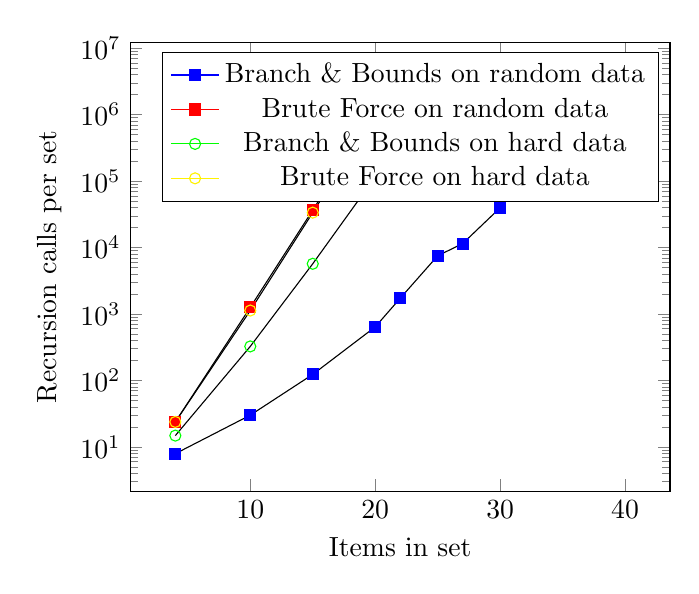
\begin{tikzpicture}
		\begin{semilogyaxis}[
			xlabel=Items in set,
			ylabel=Recursion calls per set,
			scatter/classes={
				NSm={mark=square*,blue},
				NSt={mark=square*,red},
				ZSm={mark=o,draw=green},
				ZSt={mark=o,draw=yellow}
				}
			]
			\addplot[scatter,%
				scatter src=explicit symbolic]%
			table[meta=label] {
				x y label
				4 23.71 NSt
				10 1258.43 NSt
				15 36477.82 NSt
				20 1139944.81 NSt
			};
			\addplot[scatter,%
				scatter src=explicit symbolic]%
			table[meta=label] {
				x y label
				4 7.88 NSm
				10 29.96 NSm
				15 122.98 NSm
				20 637.70 NSm
				22 1718.99 NSm
				25 7495.38 NSm
				27 11446.80 NSm
				30 39577.47 NSm
				32 145111.69 NSm
				35 320850.22 NSm
				37 782664.08 NSm
				40 3304721.06 NSm
			};
			\addplot[scatter,%
				scatter src=explicit symbolic]%
			table[meta=label] {
				x y label
				4 23.70 ZSt
				10 1125.09 ZSt
				15 33469.84 ZSt
				20 1054059.56 ZSt
			};
			\addplot[scatter,%
				scatter src=explicit symbolic]%
			table[meta=label] {
				x y label
				4 14.75 ZSm
				10 324.50 ZSm
				15 5685.97 ZSm
				20 115219.09 ZSm
				22 358548.04 ZSm
				25 2238413.90 ZSm
			};
			\addlegendentry{Branch \& Bounds on random data}
			\addlegendentry{Brute Force on random data}
			\addlegendentry{Branch \& Bounds on hard data}
			\addlegendentry{Brute Force on hard data}
		\end{semilogyaxis}
	\end{tikzpicture}
\caption{Number of recursion calls depending on number of items in set}
\label{plot:fullCalls}
\end{figure}
\begin{figure}
	\centering
	\pgfplotsset{every axis legend/.append style={
		at={(1.05,0.5)},
		anchor=west}}
	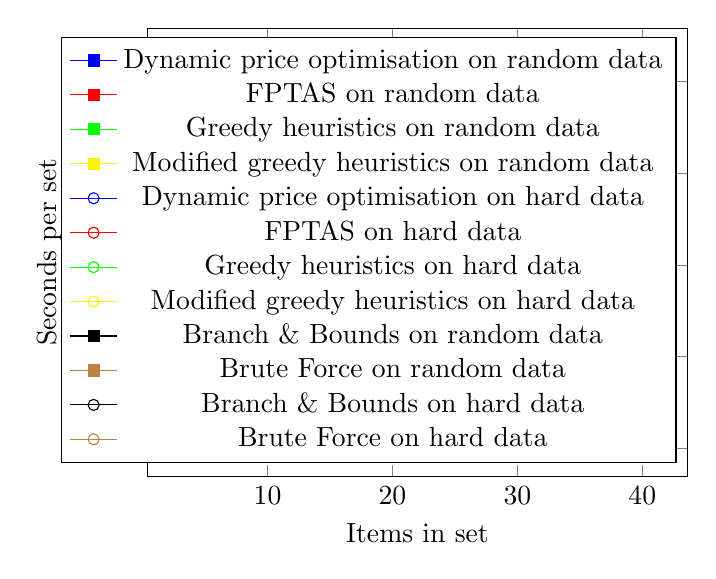
\begin{tikzpicture}
		\begin{semilogyaxis}[
			xlabel=Items in set,
			ylabel=Seconds per set,
			scatter/classes={
				dynN={mark=square*,blue},
				fptasN={mark=square*,red},
				singleN={mark=square*,green},
				hungryN={mark=square*,yellow},
				dynH={mark=o,blue},
				fptasH={mark=o,red},
				singleH={mark=o,green},
				hungryH={mark=o,yellow},
				NSm={mark=square*,black},
				NSt={mark=square*,brown},
				ZSm={mark=o,draw=black},
				ZSt={mark=o,draw=brown}
				}
			]
			\addplot[scatter,%
				scatter src=explicit symbolic]%
			table[meta=label] {
				x y label
				4 .000012 dynN
				10 .000514 dynN
				15 .014872 dynN
				20 .078888 dynN
				22 .114784 dynN
				25 .208052 dynN
				27 .223608 dynN
				30 .291732 dynN
				32 .348044 dynN
				35 .434604 dynN
				37 .547092 dynN
				40 .704324 dynN
			};
			\addplot[scatter,%
				scatter src=explicit symbolic]%
			table[meta=label] {
				x y label
				4 .000010 fptasN
				10 .000144 fptasN
				15 .000690 fptasN
				20 .001822 fptasN
				22 .002398 fptasN
				25 .003606 fptasN
				27 .004508 fptasN
				30 .006790 fptasN
				32 .008502 fptasN
				35 .011454 fptasN
				37 .013754 fptasN
				40 .017528 fptasN
			};
			\addplot[scatter,%
				scatter src=explicit symbolic]%
			table[meta=label] {
				x y label
				4 .000002 hungryN
				10 .000004 hungryN
				15 .000008 hungryN
				20 .000010 hungryN
				22 .000010 hungryN
				25 .000012 hungryN
				27 .000012 hungryN
				30 .000010 hungryN
				32 .000012 hungryN
				35 .000012 hungryN
				37 .000012 hungryN
				40 .000014 hungryN
			};
			\addplot[scatter,%
				scatter src=explicit symbolic]%
			table[meta=label] {
				x y label
				4 .000004 singleN
				10 .000004 singleN
				15 .000010 singleN
				20 .000012 singleN
				22 .000012 singleN
				25 .000012 singleN
				27 .000014 singleN
				30 .000016 singleN
				32 .000016 singleN
				35 .000016 singleN
				37 .000018 singleN
				40 .000020 singleN
			};
			\addplot[scatter,%
				scatter src=explicit symbolic]%
			table[meta=label] {
				x y label
				4 .000010 dynH
				10 .000504 dynH
				15 .014208 dynH
				20 .080942 dynH
				22 .120590 dynH
				25 .204710 dynH
				27 .249138 dynH
				30 .349580 dynH
				32 .435896 dynH
				35 .558234 dynH
				37 .649110 dynH
				40 .792216 dynH
			};
			\addplot[scatter,%
				scatter src=explicit symbolic]%
			table[meta=label] {
				x y label
				4 .000010 fptasH
				10 .000160 fptasH
				15 .000668 fptasH
				20 .001884 fptasH
				22 .002534 fptasH
				25 .004014 fptasH
				27 .005196 fptasH
				30 .007330 fptasH
				32 .009300 fptasH
				35 .012524 fptasH
				37 .014686 fptasH
				40 .019922 fptasH
			};
			\addplot[scatter,%
				scatter src=explicit symbolic]%
			table[meta=label] {
				x y label
				4 .000002 hungryH
				10 .000004 hungryH
				15 .000008 hungryH
				20 .000010 hungryH
				22 .000010 hungryH
				25 .000012 hungryH
				27 .000012 hungryH
				30 .000016 hungryH
				32 .000012 hungryH
				35 .000014 hungryH
				37 .000016 hungryH
				40 .000016 hungryH
			};
			\addplot[scatter,%
				scatter src=explicit symbolic]%
			table[meta=label] {
				x y label
				4 .000002 singleH
				10 .000006 singleH
				15 .000010 singleH
				20 .000014 singleH
				22 .000014 singleH
				25 .000014 singleH
				27 .000016 singleH
				30 .000016 singleH
				32 .000018 singleH
				35 .000018 singleH
				37 .000020 singleH
				40 .000022 singleH

			};
			\addplot[scatter,%
				scatter src=explicit symbolic]%
			table[meta=label] {
				x y label
				4 23.71 NSt
				10 1258.43 NSt
				15 36477.82 NSt
				20 1139944.81 NSt
			};
			\addplot[scatter,%
				scatter src=explicit symbolic]%
			table[meta=label] {
				x y label
				4 7.88 NSm
				10 29.96 NSm
				15 122.98 NSm
				20 637.70 NSm
				22 1718.99 NSm
				25 7495.38 NSm
				27 11446.80 NSm
				30 39577.47 NSm
				32 145111.69 NSm
				35 320850.22 NSm
				37 782664.08 NSm
				40 3304721.06 NSm
			};
			\addplot[scatter,%
				scatter src=explicit symbolic]%
			table[meta=label] {
				x y label
				4 23.70 ZSt
				10 1125.09 ZSt
				15 33469.84 ZSt
				20 1054059.56 ZSt
			};
			\addplot[scatter,%
				scatter src=explicit symbolic]%
			table[meta=label] {
				x y label
				4 14.75 ZSm
				10 324.50 ZSm
				15 5685.97 ZSm
				20 115219.09 ZSm
				22 358548.04 ZSm
				25 2238413.90 ZSm
			};
			\addlegendentry{Dynamic price optimisation on random data}
			\addlegendentry{FPTAS on random data}
			\addlegendentry{Greedy heuristics on random data}
			\addlegendentry{Modified greedy heuristics on random data}
			\addlegendentry{Dynamic price optimisation on hard data}
			\addlegendentry{FPTAS on hard data}
			\addlegendentry{Greedy heuristics on hard data}
			\addlegendentry{Modified greedy heuristics on hard data}
			\addlegendentry{Branch \& Bounds on random data}
			\addlegendentry{Brute Force on random data}
			\addlegendentry{Branch \& Bounds on hard data}
			\addlegendentry{Brute Force on hard data}
		\end{semilogyaxis}
	\end{tikzpicture}
\caption{Time needed depending on number of items in set}
\label{plot:fullTime}
\end{figure}


\section{Implementation}
Both of the algorithms are implemented with the use of recursion as it was easier to implement. However, it might be slightly less efficient than the iterative implementation, which might reflect on results.

Both of these algorithms are implemented in Python 3.7, and all data were gathered on the Windows 10 OS running on Intel(R) Core(TM) i7-6700HQ CPU @ 2.60GHz.

From \cref{plot:fullCalls} and \cref{plot:fullTime}, we can also see the direct proportionality between time and number of recursion calls.

\subsection{Brute force}
While using the naive brute force algorithm, we will check all combinations and evaluate if any of them matches the requirements. This is accomplished by creating a virtual binary tree, for example with the use of recursion, where we either insert an element or not. This approach will result in a binary tree, whose leaves will contain all possible combinations of our items.

\newpage
Afterwards, all we need to do is to validate each leaf for our conditions (maximal weight and minimal value). If at least one element matches set conditions, we can declare the problem to be solved and use any of these combinations as a certificate for our solution. In a case, where none of the leaves matches our conditions, we can declare the problem solved and use all these combinations as proof of inexisting combination matching our conditions. However, for our purpose, we have decided to stop searching once one of the elements matching our conditions was found.

This algorithm is of the $\mathbb{O}(2^n)$ complexity, which can be deduced from the worst possible combinations, where our recursion was called $2*2^n-1$, where both $2$ and $-1$ are constants thus are obsolete, which leads to the final $\mathbb{O}(2^n)$.  This complexity can also be deduced from the definition of a binary tree, from which we can get the maximal number of nodes given a level.

\subsection{Branch and bounds}
Branch and bounds method is optimised version of the brute force algorithm. In this method, we are limiting the number of combinations we need to test in two ways. The first optimisation we are using is stoping further attempts once the total weight of the items used is greater than the capacity of our knapsack.

In the second optimisation, we are comparing the value we are attempting to achieve and the value which we can still achieve given our current combination. To get the value which we can still achieve, we take the value of our current combination and add the sum of the values of all the remaining elements, which are yet to be considered for the current combination.

The complexity of this algorithm is also $\mathbb{O}(2^n)$, as in the worst case, such as when we get a list of elements with low weight and low value with the last element of high weight and value, we are forced to go through all of the possible combinations to ensure none of them is viable for our requirements. However, if we take a look at \cref{plot:fullCalls} and \cref{plot:fullTime}, we can see the improvement for the average complexity, which was lowered considerably. On the other hand, if we take a look at the hard dataset, the improvement is visible, but not sufficient to show any substantial impact.

% \section{Comparison}
% For comparison of these two algorithms, we have used two sets of data. The first set contains randomly generated data, which have been marked as squares in \cref{plot:fullCalls} and \cref{plot:fullTime}.

% The second dataset contains data generated purposefully to be hard to resolve. Results from applying both our algorithms have been marked with circles in \cref{plot:fullCalls} and \cref{plot:fullTime}.

% \subsection{Configurations}

% \subsection{Time}


\section{Histograms}
When we take a look at the histograms in \cref{plot:detailStupidNormal,plot:detailSmartNormal,plot:detailStupidHard,plot:detailSmartHard}, we can see the improvement on both the normal and the hard datasets. For both of the datasets, we can see the curve for the branch and bounds algorithm to approximately match the normal distribution as we could expect. On the other hand, histograms for the brute force solutions focus its values near the higher bound of the complexity, as there are nearly no optimisations to allow us to achieve a better result.

\begin{figure}
	\centering
	\pgfplotsset{every axis legend/.append style={
		at={(1.05,0.5)},
		anchor=west}}
	\begin{tikzpicture}
        \begin{axis}[
			xlabel=Recursions called,
			ylabel=Count,
            axis on top,
            ybar interval,
            x tick label as interval=false,
            xtick={},
            grid=none
        ]

        \addplot+[hist={data=x}]
        file {data/dataSetDetailCalls_stupid.txt};
		\end{axis}
	\end{tikzpicture}
\caption{Histogram for normal data set of 4 elements per instance with brute force algorithm}
\label{plot:detailStupidNormal}
\end{figure}

\begin{figure}
	\centering
	\pgfplotsset{every axis legend/.append style={
		at={(1.05,0.5)},
		anchor=west}}
	\begin{tikzpicture}
        \begin{axis}[
			xlabel=Recursions called,
			ylabel=Count,
            axis on top,
            ybar interval,
            x tick label as interval=false,
            xtick={},
            grid=none
        ]

        \addplot+[hist={data=x}]
        file {data/dataSetDetailCalls_smart.txt};
		\end{axis}
	\end{tikzpicture}
\caption{Histogram for normal data set of 4 elements per instance with B\&B algorithm}
\label{plot:detailSmartNormal}
\end{figure}

\begin{figure}
	\centering
	\pgfplotsset{every axis legend/.append style={
		at={(1.05,0.5)},
		anchor=west}}
	\begin{tikzpicture}
        \begin{axis}[
			xlabel=Recursions called,
			ylabel=Count,
            axis on top,
            ybar interval,
            x tick label as interval=false,
            xtick={},
            grid=none
        ]

        \addplot+[hist={data=x}]
        file {data/dataSetDetailCallsHard_stupid.txt};
		\end{axis}
	\end{tikzpicture}
\caption{Histogram for hard data set of 4 elements per instance with brute force algorithm}
\label{plot:detailStupidHard}
\end{figure}

\begin{figure}
	\centering
	\pgfplotsset{every axis legend/.append style={
		at={(1.05,0.5)},
		anchor=west}}
	\begin{tikzpicture}
        \begin{axis}[
			xlabel=Recursions called,
			ylabel=Count,
            axis on top,
            ybar interval,
            x tick label as interval=false,
            xtick={},
            grid=none
        ]

        \addplot+[hist={data=x}]
        file {data/dataSetDetailCallsHard_smart.txt};
		\end{axis}
	\end{tikzpicture}
\caption{Histogram for hard data set of 4 elements per instance with B\&B algorithm}
\label{plot:detailSmartHard}
\end{figure}

\section{Conclusion}
In conclusion, we have created two implementations for solving the decision version of the 0/1 knapsack problem. We have compared the efficiency of these two implementations (brute force and the branch and bounds optimisation) with respect to processor time and the number of recursion calls. Moreover, we have also compared histograms for two datasets (randomly generated data and purposefully hard data), each for both of our algorithms, showing their complexity and standard behaviour as well as extreme cases.

\newpage
\bibliographystyle{iso690}
% \bibliographystyle{csn690}
% \bibliography{mybibliographyfile}
\nocite{*} % all entries in the bib file
\bibliography{database.bib}

\end{document}